\section{Introduction} \label{sec:introduction}
%$$$$$$$$$$$$$$$$$$$$$$$$$$$$$$$$$$$$$$$$$$$$$$$$$$$$$$$$$$$$$$$$$$$$$$$$$$$$$$$$
%$$$$$$$$$$$$$$$$$$$$$$$$$$$$$$$$$$$$$$$$$$$$$$$$$$$$$$$$$$$$$$$$$$$$$$$$$$$$$$$$
%Background : 스파크 -> cloud가 아닌 scale-up server 에서의 scalability에 대한 연구가 필요해짐
%$$$$$$$$$$$$$$$$$$$$$$$$$$$$$$$$$$$$$$$$$$$$$$$$$$$$$$$$$$$$$$$$$$$$$$$$$$$$$$$$
%빅데이터 처리하는데 많이 사용되는 framework 중 하나는 스파크이다.
Popular big data analytics infrastructures(e.g, Spark~\cite{Zaharia2012RDD},
Hadoop~\cite{Shvachko2010HDF}) have been developed for a cluster scale-out
environment, which adds nodes to a cluster system.
On the other hand, scale-up environment, which adds resources(e.g, cpu, memory)
to a single node system, only special-purpose techniques exist.
In science and machine learning fields, researchers
commonly used scale-up server environments, and they now need big data analytics
frameworks~\cite{Chaimov2016SSH}.
Moreover, hardware trends are beginning to change for the scale-up
server; a scale-up server can now have substantial CPU, memory,
and storage I/O resources~\cite{Appuswamy2013SVS}.
Therefore, the big data analytics infrastructure on scale-up server is
also important.

%$$$$$$$$$$$$$$$$$$$$$$$$$$$$$$$$$$$$$$$$$$$$$$$$$$$$$$$$$$$$$$$$$$$$$$$$$$$$$$$$
%$$$$$$$$$$$$$$$$$$$$$$$$$$$$$$$$$$$$$$$$$$$$$$$$$$$$$$$$$$$$$$$$$$$$$$$$$$$$$$$$
%Problem : scale-up server에서 시스템으로 구성된 scalability가 없음 
% 2가지 관련 연구가 있음.
% 1. 24코어 이하의 서버에서의 Scalability 분석을 하였으나 해결책을 제안하지 않았음.
% 2. HPC(100이상) 으로 분석하였으나 flie system 관점으로 분석하였음.:메인 병목지점은 파일 시스템
% 3. Scalable한 파일 시스템을 사용한 후 Scalability에 대한 분석한 결과와 해결방법은 없음.
Spark is one of widely used big data analytics framework.
However, Spark has been reported that it does
not scale on the single node scale-up server because of garbage
collection(GC)
overhead~\cite{Ahsan2016SVS}~\cite{Ousterhout2015MSP}~\cite{Maas2016THL} and
locality of memory accesses on Non-Uniform Memory Access(NUMA)
architecture~\cite{Cao2016ADS}.
Therefore, A.J. Awan \textit{et al.} analysed GC time and compared state of the art
garbage collectors by changing the GC.
Moreover, in order to avoid high costs of remote memory access, researchers have
attempted to create a new NUMA balancing~\cite{Dashti2013TMH}~\cite{AutoNUMA}, but
these methods also can not satisfactory compared to partitioning approch(see section~\ref{sec:scale}).


%$$$$$$$$$$$$$$$$$$$$$$$$$$$$$$$$$$$$$$$$$$$$$$$$$$$$$$$$$$$$$$$$$$$$$$$$$$$$$$$$
%본 연구에서 분석한 결과와 제안하는 방법으로 향상된 성능
%$$$$$$$$$$$$$$$$$$$$$$$$$$$$$$$$$$$$$$$$$$$$$$$$$$$$$$$$$$$$$$$$$$$$$$$$$$$$$$$$
%$$$$$$$$$$$$$$$$$$$$$$$$$$$$$$$$$$$$$$$$$$$$$$$$$$$$$$$$$$$$$$$$$$$$$$$$$$$$$$$$
Our goals is to reduce the GC and the memory access latency overheads that
have been a major problem of Spark scalability.
To achieve our goal, this paper presents a new partitioning method that
eliminates the GC and remote access overheads by applying
Docker container-based efficient partitioning for Spark on scale-up
server.
Our basic key idea is that shared-memory system is dealt with as the
distributed-system using partitioning approach in order to eliminate GC and
memory access overheads.
We use Docker containers since the overhead of a Docker
container is much smaller than a traditional virtual
machine~\cite{Merkel2014DLL} and the container-based approach can easily combine
existing container management solutions such as Google Borg~\cite{Borg} and
Kubernets~\cite{Kubernetes}.

Our method make shared resource to small size group as much as
possible(minimal partition value is per-socket) because prior work have showed
that shared resource contention should be minimized by partitioning shared
resource accesses~\cite{Qureshi2006UCP}.
Small size cpu groups can mitigate the thread serialized problem cased by GC
pause time, and these group may only access to local NUMA memory.
Moreover, partitioning method can somewhat reduce the operating systems
scalability problems(e.g, address space
problem ~\cite{AustinTClements2012RCUBalancedTrees}~\cite{Clements2013RadixVM},
cache communication overhead~\cite{SilasBoydWickizerPth}~\cite{Hendler2010FC})

%$$$$$$$$$$$$$$$$$$$$$$$$$$$$$$$$$$$$$$$$$$$$$$$$$$$$$$$$$$$$$$$$$$$$$$$$$$$$$$$$
%본 연구에서 분석한 결과와 제안하는 방법으로 향상된 성능
%$$$$$$$$$$$$$$$$$$$$$$$$$$$$$$$$$$$$$$$$$$$$$$$$$$$$$$$$$$$$$$$$$$$$$$$$$$$$$$$$
%$$$$$$$$$$$$$$$$$$$$$$$$$$$$$$$$$$$$$$$$$$$$$$$$$$$$$$$$$$$$$$$$$$$$$$$$$$$$$$$$
To evaluate our approach, we applied our partitioning method on 120 core
scale-up server.
A too small size partitioning may reduce GC overhead and remote memory access,
but the benefits do not come for free because it may cause straggler tasks
problem~\cite{Ousterhout2015MSP}~\cite{Ren2015HDS}.
Thus, this paper additionally describes performance scalability
depending on partitioning size.
Evaluation of the proposed best-fit partitioning on a 120 core system
 reveals that the execution times could be improved by 1.6x, 1.7x, 1.5x and 1.1x
 for Word Count, Naive Basian, Grep and K-means, respectively.

%$$$$$$$$$$$$$$$$$$$$$$$$$$$$$$$$$$$$$$$$$$$$$$$$$$$$$$$$$$$$$$$$$$$$$$$$$$$$$$$$
%본 연구에서 기여한 것 : 
% 1. 100코어 이상의 scale-up 서버에서의 scalability 측정 및 분석
% 2. 도커 파티션 기법을 활용한 scalability 향상 방법 제안
%$$$$$$$$$$$$$$$$$$$$$$$$$$$$$$$$$$$$$$$$$$$$$$$$$$$$$$$$$$$$$$$$$$$$$$$$$$$$$$$$

\textbf{Contributions.} Our research makes the following contributions:
\begin{itemize}
\item 
We analyzed Apache Spark performance scalability on 120 core scale-up server.
The results of scalability was that parallel GC can improve performance
scalability up to 60 core, but then the GC flattens out after 60 core.
\item 
We evaluated proposal partitioning approach on a manycore scale-up
server thereby mitigating scale-up server scalability problems in BigDataBench.
Our approach improved throughput and execution time from 1.1x through
1.7x on 120 core.
\end{itemize}


\begin{figure*}[tb]
    \centering
    \begin{subfigure}[b]{0.25\textwidth}
        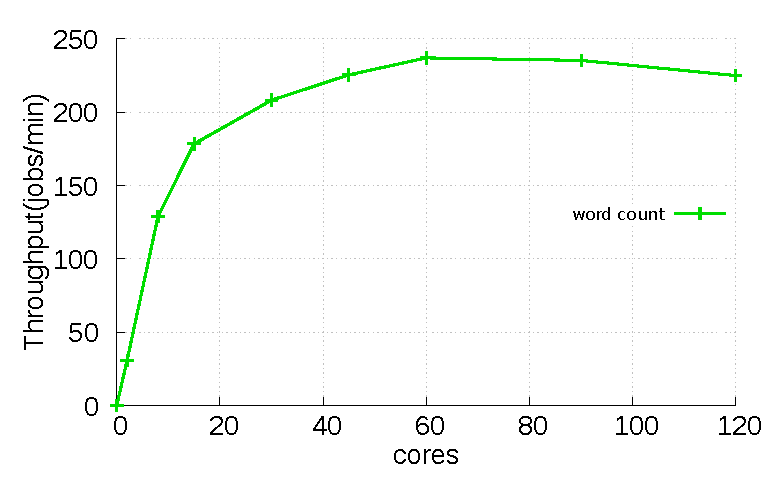
\includegraphics[width=1.8in]{graph/wc.eps}
        \caption{Word Count}
    \end{subfigure}%
    \begin{subfigure}[b]{0.25\textwidth}
        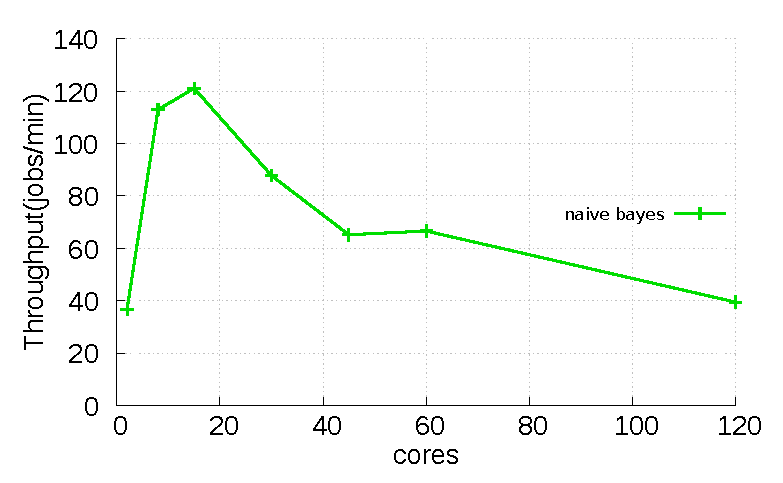
\includegraphics[width=1.8in]{graph/nb.eps}
        \caption{Naive Basian}
    \end{subfigure}%
    \begin{subfigure}[b]{0.25\textwidth}
        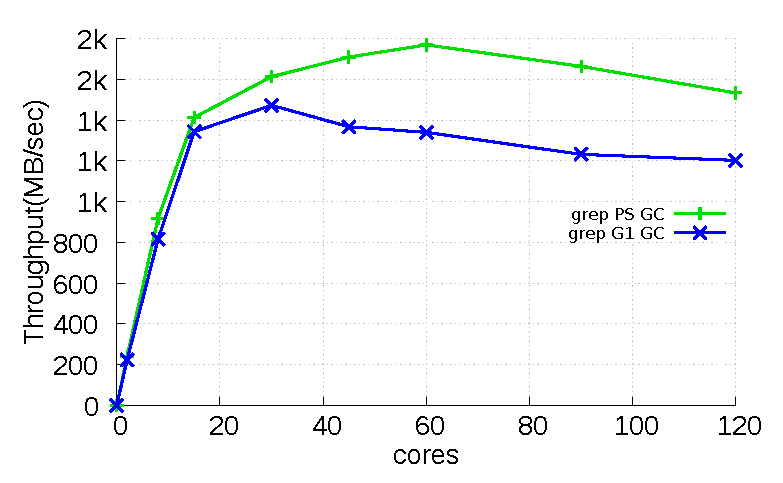
\includegraphics[width=1.8in]{graph/grep.eps}
        \caption{Grep}
    \end{subfigure}%
    \begin{subfigure}[b]{0.25\textwidth}
        \includegraphics[width=1.8in]{graph/kmeans.eps}
        \caption{K-means}
    \end{subfigure}%
    \caption{Performance scalability on 120 core.}
    \label{fig:utilization}
\end{figure*}



\begin{figure*}[tb]
    \centering
    \begin{subfigure}[b]{0.25\textwidth}
        \includegraphics[width=1.8in]{graph/wc_cpuutils.eps}
        \caption{Word Count}
    \end{subfigure}%
    \begin{subfigure}[b]{0.25\textwidth}
        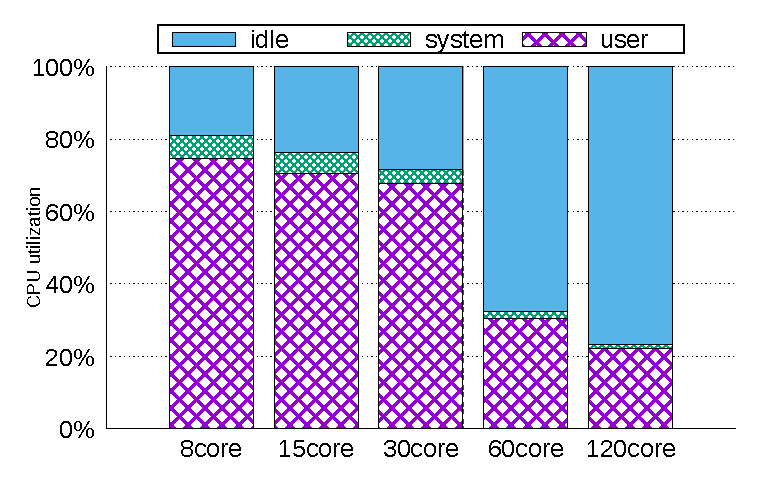
\includegraphics[width=1.8in]{graph/nb_cpuutils.eps}
        \caption{Naive Basian}
    \end{subfigure}%
    \begin{subfigure}[b]{0.25\textwidth}
        \includegraphics[width=1.8in]{graph/grep_cpuutils.eps}
        \caption{Grep}
    \end{subfigure}%
    \begin{subfigure}[b]{0.25\textwidth}
        \includegraphics[width=1.8in]{graph/kmeans_cpuutils.eps}
        \caption{K-means}
    \end{subfigure}%
        \centering
    \caption{CPU utilization on 120 core.}
    \label{fig:cpuutilization}
\end{figure*}

%$$$$$$$$$$$$$$$$$$$$$$$$$$$$$$$$$$$$$$$$$$$$$$$$$$$$$$$$$$$$$$$$$$$$$$$$$$$$$$$$
%$$$$$$$$$$$$$$$$$$$$$$$$$$$$$$$$$$$$$$$$$$$$$$$$$$$$$$$$$$$$$$$$$$$$$$$$$$$$$$$$
%Mapping
%$$$$$$$$$$$$$$$$$$$$$$$$$$$$$$$$$$$$$$$$$$$$$$$$$$$$$$$$$$$$$$$$$$$$$$$$$$$$$$$$
The rest of this paper is organized as follows.
Section 2 describes the test-bed and Spark scalability problem.
Section 3 describes the our partitioning approach and 
Section 4 shows the results of the experimental evaluation. 
Section 5 describes related works. 
Finally, section 6 concludes the paper.

